\documentclass{article}
\usepackage[a4paper,margin=1in]{geometry}
\usepackage{amsmath, amsfonts, amssymb, amstext, mathtools, stmaryrd, textcomp, xcolor, graphicx, tikz}
\usepackage[hidelinks]{hyperref}
\usetikzlibrary{automata, positioning, arrows, trees}
\tikzset{->,>=stealth,
every state/.style={thick, fill=gray!10}, 
initial text=$ $,
}
\newcommand{\answer}{\textcolor{red}}
\newcommand{\e}{\varepsilon}
\newcommand{\s}{\Sigma}
\newcommand{\g}{\Gamma}
\newcommand{\so}{\rightarrow}
\newcommand{\str}{\texttt}
\newcommand{\newp}{\\[2mm]}
\newcommand{\defeq}{\coloneqq}
\newcommand{\spc}{\textvisiblespace}

\title{Homework 08}
\author{Aaron Wang}
\date{April 29 2025}

\begin{document}
\maketitle
\begin{enumerate}
    \item Define a \emph{neural network} with $l$ inputs and $m$ hidden units to be a function that takes a sequence of inputs  $x_1, \ldots, x_l \in \{0, 1\}$ and computes
    \begin{align*}
        \displaystyle
        h_j &= H\Big(\sum_{i=1}^lx_iu_{i,j}+a_j\Big) & j = 1,\ldots,m\\
        y &= H\Big(\sum_{j=1}^mh_jv_j+b\Big)
    \end{align*}
    where
    \[
        H(x) = 
        \begin{cases}
            1 & \text{if } x > 0\\
            0 & \text{otherwise}
        \end{cases}
    \]
    The weights $u_{i,j}$ , $a_j$ , $v_j$ , and $b$ can be any rational numbers, and they don’t depend on $x_1, \ldots, x_l$. Let’s say that the size of the neural network is the number of units $(n = l + m + 1)$.
    Prove that it is NP-complete to decide, given a neural network with $l$ inputs, whether there is any sequence of inputs $x_1, \ldots, x_l$ that makes $y = 1$.\newp
    \answer{
    Let NEURAL$ = \{ \langle N \rangle \:|\: N$ is a \emph{neural network} and there exists inputs $x_1,...,x_l$ that make $y = 1\}$.\newp
    % To prove NEURAL is NP-complete, we must show it is both NP and NP-hard.\newp
    Let $V$ be a verifier for NEURAL.\newp
    $V =$ ``On input $\langle N, X \rangle$ where $N$ is a neural network and $X$ is the sequence of inputs $x_1,...,x_l$:
    \begin{enumerate}
        \item [1.] $\forall j$ solve $h_j$.
        \item [2.] Solve $y$.
        \item [3.] If $y = 1$, \emph{accept}; otherwise, \emph{reject}.
    \end{enumerate}
    Step 1 is $\mathcal{O}(l*m)$ and step 2 is $\mathcal{O}(m)$. Consequently, $V$ is definitely $\mathcal{O}(n^2)$. Since we have a deterministic polynomial time verifier, we know NEURAL is NP.\newp
    Here are the details of a reduction from 3SAT to NEURAL that operates in polynomial time.
    \begin{enumerate}
        \item [1.] Initialize nodes for $x_i$ and $\overline{x_i}$ s.t. they must be opposites. For each variable $x_i$:
        \begin{itemize}
            \item Create nodes $x_i$ and $x_{-i}$
            \item Create node $h_{x_i} = H(x_i+x_{-i})$
            \item Create node $h_{x_{-i}} = H(-x_i-x_{-i}+2)$
        \end{itemize}
        \item [2.] Translate all the clauses into the neural network. For each clause $j$: create $h_j$ s.t. 
        \begin{itemize}
            \item if $x_i$ is in the clause, $u_{i,j} = 1$
            \item if $\overline{x_i}$ is in the clause, $u_{-i,j} = 1$
            \item otherwise $u_{i,j} = 0$
        \end{itemize}
        \item [3.] And every clause (step 2) and restriction (step 1) together. $\displaystyle y = H(\sum_{j=1}^mh_j - m + 1)$
    \end{enumerate}
    Following this reduction, we have mapped each boolean expression to a neural network that is satisfiable iff the boolean expression is. Every $N$ that is made from this reduction will only be satisfiable, if there is a series of inputs that make every $h = 1$ or all clauses and restrictions are satisfied 
    Step 1 is $\mathcal{O}(n)$, 2 is $\mathcal{O}(n^2)$, and 3 is $\mathcal{O}(n)$. This is clearly a $\mathcal{O}(n^2)$ reduction so NEURAL is NP-Hard.\newp
    Since NEURAL is NP and NP-Hard, it is NP-complete.
}
\newpage
    \item In the game of Digits, you are given
    \begin{itemize}
        \item A target number $t$ (e.g., 56)
        \item A multiset $S$ of source numbers (e.g. $\{2, 3, 4, 5, 10, 25\}$)
        \item A set of $\mathcal{O}$ of operations ($\{+,-,\times,\div\}$)
    \end{itemize}
    and the goal is to write an expression involving the source numbers, operations, and parentheses that evaluates to the target number. You don’t have to use every number, but each number can only be used as many times as it occurs in $S$. If this possible, we say that ($t$, $S$, $\mathcal{O}$) is solvable. For example, ($56, \{2, 3, 4, 5, 10, 25\, \{+, -, \times, \div \}$) is solvable because
    \[
    2 \times 4 \times (10 - 3) = 56
    \]
    Prove that $\{+, \times \}$-DIGITS is NP-complete:
    \[
        \{+, \times \}\text{-DIGITS} = \{\langle t, S \rangle | (t, S, \{+, \times \}) \text{ is solvable} \}.
    \]
    Assume that the size of $\langle t, S\rangle$ is the total number of bits in $t$ and $S$.\newp
    \answer{
The intuition for the following conversion is this. Use the 2 stacks in the same way as the tape would be used where the first stack is used to hold everything preceding the head and the other stack holds everything following and where the head is currently looking at the top element on the second stack. The head moves right by moving one element from the second stack to the first stack, and moves left by moving an element from the first stack to the second. 
To consider the edge case of moving left when all the way at the left already, you check for a $\$$ and in that case, you move back right.
To consider the edge case, where we extend pass the starting string (go to trailing spaces), we would
Let $M$ be a TM.\newp
Let $P = \{Q,\s,\g, \delta, s, F\}$ be the 2PDA such that
\begin{quote}
\begin{enumerate}
    \item [1.] The string ($\s$) alphabet is the same as that of $M$.
    \item [2.] $\g = \s \cup \{\text{\spc, \str{\$}}\}$. The stack alphabet is string alphabet with \spc \:and \str{\$}. 
    \item [3.] Have pre-processing states to read the input onto the stack and add \str{\$} to demarcate the end and beginning. $\forall a \in \s$.\footnote{The outgoing transition from $s_2$ will be $\e$, $\e$, $\e \rightarrow \e$, $\e$ into the original start state }
    \begin{figure}[h]
\centering
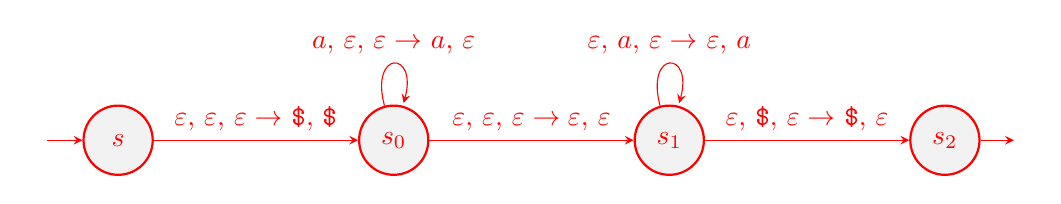
\begin{tikzpicture}
\color{red}
    \node[state, initial] (q0) {$s$};
    \node[state, xshift=3.5cm] (q1) {$s_0$};
    \node[state, xshift=7cm] (q2) {$s_1$};
    \node[state, xshift=10.5cm] (q3) {$s_2$};
    \node[draw=none, xshift=11.5cm] (phantom) {};

    \draw
    (q0) edge[] node[above]{$\e$, $\e$, $\e \rightarrow$ \str{\$}, \str{\$}}(q1)
    (q1) edge[loop above] node[above]{$a$, $\e$, $\e \rightarrow$ $a$, $\e$} (q1)
    (q1) edge[] node[above]{$\e$, $\e$, $\e \rightarrow \e$, $\e$}(q2)
    (q2) edge[loop above] node[above]{$\e$, $a$, $\e \rightarrow$ $\e$, $a$} (q2)
    (q2) edge[] node[above]{$\e$, \str{\$}, $\e \rightarrow$ \str{\$}, $\e$}(q3)
    (q3) edge[] node[above]{\:} (phantom)
    ;
\end{tikzpicture}
\end{figure}
    \item [4.] For each state $q$ of $M$, the same state $q$ in $P$.
    \begin{enumerate}
        \item $F = \{ q_{\text{\emph{accept}}}\}$.
        \item Additionally, to ensure rejection, make sure that there are no outgoing transitions from $q_{\text{\emph{reject}}}$.
    \end{enumerate}
    \item [5.] For each transition of $M$ s.t. $a,b \in \s \cup \{$\spc$\}$ create transitions in $P$ such that first if we are reading (trailing spaces), \$ $\rightarrow$  \spc \: and then R transitions move right and L transitions move left if possible.
\begin{enumerate}
    \item R transitions.\\
    For every transition of $M$ that looks like this\\
    \begin{figure}[h]
    \centering
    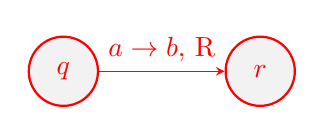
\begin{tikzpicture}
    \color{red}
        \node[state] (q_0) {$q$};
        \node[state, xshift=2.5cm] (r_0) {$r$};
    
        \draw
        (q_0) edge[] node[above]{$a \rightarrow b$, R}(r_0)
        ;
    \end{tikzpicture}
    \end{figure}\\
    Create transitions like this in $P$\\
        \begin{figure}[h]
    \centering
    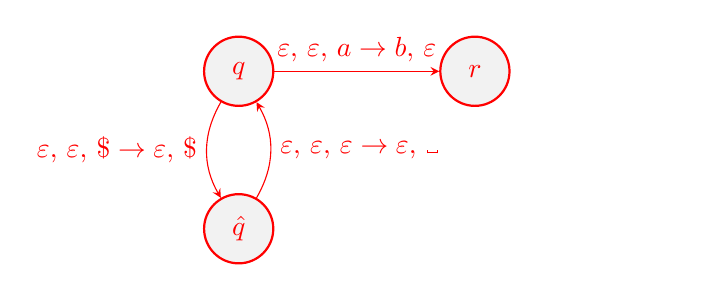
\begin{tikzpicture}
    \color{red}
        \node[state] (q_1) {$q$};
        \node[state, yshift=-2cm] (q) {$\hat{q}$};
        \node[state, xshift=3cm] (r_1) {$r$};
        \node[draw=none, xshift=5.5cm] (phantom) {};
        \draw
        (q_1) edge[] node[above]{$\e$, $\e$, $a \rightarrow b$, $\e$ }(r_1)
        (q_1) edge[bend right] node[left]{$\e$, $\e$, $\$ \rightarrow \e$, $\$$ }(q)
        (q) edge[bend right] node[right]{$\e$, $\e$, $\e \rightarrow \e$, \spc }(q_1)
        ;
    \end{tikzpicture}
    \end{figure}
    \item L transitions.\\
    For every transition of $M$ that looks like this\\
    \begin{figure}[h]
    \centering
    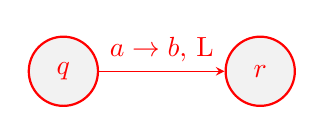
\begin{tikzpicture}
    \color{red}
        \node[state] (q_0) {$q$};
        \node[state, xshift=2.5cm] (r_0) {$r$};
    
        \draw
        (q_0) edge[] node[above]{$a \rightarrow b$, L}(r_0)
        ;
    \end{tikzpicture}
    \end{figure}\\
    Create transitions like this in $P$ $\forall c \in \s \cup \{$\spc$\}$ 
    \begin{figure}[h!]
    \centering
    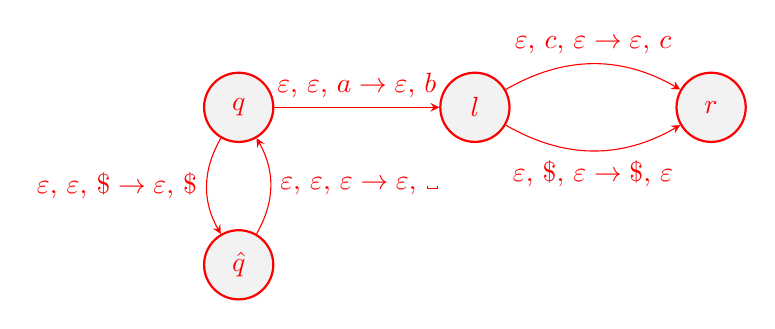
\begin{tikzpicture}
    \color{red}
        \node[state] (q_1) {$q$};
        \node[state, yshift=-2cm] (q) {$\hat{q}$};
        \node[state, xshift=3cm] (l) {$l$};
        \node[state, xshift=6cm] (r) {$r$};
        \draw
        (q_1) edge[] node[above]{$\e$, $\e$, $a \rightarrow \e$, $b$ }(l)
        (q_1) edge[bend right] node[left]{$\e$, $\e$, $\$ \rightarrow \e$, $\$$ }(q)
        (q) edge[bend right] node[right]{$\e$, $\e$, $\e \rightarrow \e$, \spc }(q_1)
        (l) edge[bend left] node[above]{$\e$, $c$, $\e \rightarrow \e$, $c$ }(r)
        (l) edge[bend right] node[below]{$\e$, $\$$, $\e \rightarrow \$$, $\e$ }(r)
        ;
    \end{tikzpicture}
    \end{figure}
\end{enumerate}
    \item [6.] $Q$ is the set of all the states we created.
    \begin{enumerate}
        \item The states from pre-processing $s$, $s_0$, $s_1$ and $s_2$.
        \item The states copied from the $M$.
        \item The new states $\hat{q}$ and $l$ defined by the transitions (for every transition).
    \end{enumerate}
\end{enumerate}
\end{quote}
}
\newpage
    \item You are at the entrance to a room whose floor is made entirely of trapdoors, and underneath the floor is a pool of lava. Each trapdoor is either open or closed.\newp
    At the entrance to the room is a control panel that has buttons labeled with symbols. For any symbol $\sigma$, if you push the button labeled $\sigma$, then all the trapdoors labeled $\sigma$ that are closed become open, and all the trapdoors labeled $\sigma$ that are open become closed. \newp
    In general, a room can be any size rectangle, with an entrance and exit anywhere around the perimeter, any initial pattern of open/closed trapdoors, and any number of labels/buttons.\newp
    Prove that it is NP-complete to decide, given a room as defined above, whether there is a subset of buttons that you can push to make a safe path from the entrance to the exit.\newp
    \answer{
Let $P$ be a $\mathcal{P}''$ program. Let us use the follow construction to create a Turing Machine $M$ that compiles $P$ into a standard single-tape TM.
\begin{quote}
\begin{enumerate}
    \item[i.] Initialize an empty stack to keep track of open loops.\footnote{At any point, if there is nothing to pop from this stack, $P$ was not a proper program. Additionally, if there are extra elements on the stack at the end, $P$ was not a proper program.}
    \item[ii.] Go through every character of the code and parse it in this way, keeping track of a counter $i$ for every character.\footnote{$i$ starts at 0, increments by 1 every time and $i,j \in \mathbb{Z}$} In the following steps, every transition created is from $q_i$ to $q_{i+1}$\\[2mm]
    \begin{tabular}{l l}
    \str{<} & $\forall j \in [0,n-1]$ Create transitions $a_j \rightarrow a_j$, L\\[2mm]
    \str{>} & $\forall j \in [0,n-1]$ Create transitions $a_j \rightarrow a_j$, R\\[2mm]
    \str{+} & $\forall j \in [0,n-2]$ Create transitions $a_j \rightarrow a_{j+1}$, S\\
    & Create transition $a_{n-1} \rightarrow a_0$, S\\[2mm]
    \str{-} & $\forall j \in [1,n-1]$ Create transitions $a_j \rightarrow a_{j-1}$, S\\
    & Create transition $a_{0} \rightarrow a_{n-1}$, S\\[2mm]
    \str{[} & Add $i$ to stack of open bracket placement.\\
    & $\forall j \in [1,n-1]$ Create transitions $a_{j} \rightarrow a_{j}$, S\\[2mm]
    \str{]} & Let $j$ be popped value from the open bracket placement stack.\\
    & Let $q_i$ = $q_j$ (create the looping state)\\
    & Create transition $a_{0} \rightarrow a_{0}$, S\\[2mm]
    \end{tabular}
    \item[iii.] $\forall q \in Q$ create a transition \spc\:$\rightarrow a_0, S$ from $q$ to itself.
    \item[iv.] Let $m$ be the length of the program $P$. $q_m$ is the final state that we have created so far. From $q_m$...
    \begin{itemize}
        \item $\forall j \in [1,n-1]$ create a transition $a_{j} \rightarrow a_{j}$, S to $q_{\text{\emph{accept}}}$.
        \item create a transition from $a_0 \rightarrow a_0$, S to $q_{\text{\emph{reject}}}$.
    \end{itemize}
\end{enumerate}
\end{quote}
The formal description of $M = \{Q, \s, \g, \delta, q_0,q_{\text{\emph{accept}}}, q_{\text{\emph{reject}}}\}:$
\begin{itemize}
    \item $Q = \{q_0,q_1...q_m,q_{\text{\emph{accept}}}, q_{\text{\emph{reject}}}\}$.
    \item $\s$ is a subset of $\g$ as defined by the directions without $a_0$ and \spc.
    \item $\g = \{a_0,...,a_{n-1},\text{\spc}\}$
    \item $\delta$ as defined above.
    \item $q_0$ as defined above.
    \item $q_{\text{\emph{accept}}}$ as defined above.
    \item $q_{\text{\emph{reject}}}$ as defined above.
\end{itemize}
}
\end{enumerate}
\end{document}